% =========================================================================
% Appendix C — Stage-3 orbital (gamma-rocket / ANTIMATTER). FILLED.
%   folds UFO/verify/stage3-orbital-gamma.md: annihilation E=2 m_p c^2,
%   relativistic exhaust -> photon I_sp ceiling c/g ~ 3.06e7 s, the honest
%   c/g-vs-spec-target gap (mass-flow definition), the F-ANTI-3 closure via
%   fuel-mass redefinition (9/9 PASS), the 3 green verify atoms verbatim,
%   atlas idempotent reuse, and a pgfplots I_sp ladder chart.
% =========================================================================
\section{Stage-3 Orbital --- Antimatter $\gamma$-Rocket and the $I_{\text{sp}}$ Ceiling}
\label{app:stage3}

This appendix is the full data record for ladder rung
\textcircled{\scriptsize 3} (orbital). It folds the
ANTIMATTER-inherited $\gamma$-rocket closed form: annihilation
$E=2m_pc^2$ ($\bar p p\!\to\!2\gamma$ leading channel), the relativistic
rocket exhaust, and the photon specific-impulse ceiling
$I_{\text{sp,max}}=c/g\approx\SI{3.06e7}{\second}$, with the three
\tierGreen\ \textsc{Supported-Numerical} atoms
(\verb|pair_threshold_total|$(938.272)=6567.904$,
\verb|rel_kinetic_from_p| at the ultra-relativistic and kinetic$=$rest
crossover) reproduced verbatim from
\texttt{UFO/verify/stage3-orbital-gamma.md}, each at $|\Delta|=0$ and
already folded into the atlas SSOT (\texttt{663698a0}) by the ANTIMATTER
parent. We honestly record the two-decade gap between the $c/g$ photon
ceiling and the spec target $I_{\text{sp}}\!\ge\!10^9$\,s as a mass-flow
definition difference (@D~d6 --- no forced target number), and note the
later F-ANTI-3 closure via fuel-mass re-definition.

% -------------------------------------------------------------------------
\subsection{Annihilation energy and the photon $I_{\text{sp}}$ ceiling}
\label{app:stage3-deriv}

In the rest frame the leading baryon--antibaryon channel is
\begin{equation}
\bar p + p \;\longrightarrow\; 2\gamma,
\qquad
E_\gamma = m_p c^2 = \SI{938.272}{\mega\electronvolt},
\qquad
E_{\text{pair}} = 2 m_p c^2 = \SI{1876.544}{\mega\electronvolt},
\label{eq:s3-annih}
\end{equation}
i.e.\ the entire rest mass converts to photons. This is the maximal
energy density of any fuel: chemical ($\sim\!\text{eV/bond}$), fission
($\sim\!0.09\%\,mc^2$), and D--T fusion ($\sim\!0.4\%\,mc^2$) all sit far
below the $100\%\,mc^2$ of matter--antimatter annihilation. The exhaust
is photons, whose speed is $c$, so the specific impulse
$I_{\text{sp}}=v_e/g$ approaches its absolute ceiling
\begin{equation}
v_e\to c
\quad\Longrightarrow\quad
I_{\text{sp,max}} = \frac{c}{g}
 = \frac{2.998\times10^8}{9.80665}
 \approx \SI{3.057e7}{\second}.
\label{eq:s3-isp}
\end{equation}
The exhaust kinematics follow the relativistic dispersion
$E^2=(pc)^2+(mc^2)^2$: a photon ($m=0$) has $E=pc$, $\beta=1$; a massive
exhaust has $\beta<1$ and stays below the ceiling. The hover/cruise/orbital
ladder spans roughly nine decades of $I_{\text{sp}}$ from chemical to the
photon ceiling (Fig.~\ref{fig:s3-isp-ladder}).

% -------------------------------------------------------------------------
\subsection{Verify atoms and verbatim verdicts}
\label{app:stage3-verify}

The relativistic energy bookkeeping is closed by three \tierGreen\ atoms
(Table~\ref{tab:s3-verify}): the annihilation-energy anchor
$\verb|pair_threshold_total|(938.272)=7\,m_pc^2=6567.904$ (the
ANTIMATTER production anchor), the ultra-relativistic exhaust regime
($\beta=0.995$, $\gamma\!\approx\!10.05$), and the kinetic$=$rest
crossover ($pc=\sqrt3\,m_pc^2\Rightarrow T=m_pc^2$, the doubling threshold
underlying the $c/g$ ceiling derivation).

\begin{table}[h]
\centering
\small
\setlength{\tabcolsep}{5pt}
\begin{tabular}{@{}l l r r r c@{}}
\toprule
\textbf{atom} & \textbf{args (MeV)} & \textbf{expected} & \textbf{observed} & $|\Delta|$ & \textbf{tier} \\
\midrule
\verb|pair_threshold_total| & $(938.272)$  & $6567.904$ & $6567.904$ & $0$ & \tierGreen \\
\verb|rel_kinetic_from_p|   & $(9382.72)$  & $8491.2449$ & $8491.2449$ & $0$ & \tierGreen \\
\verb|rel_kinetic_from_p|   & $(1625.13)$  & $938.272$  & $938.272$  & $0$ & \tierGreen \\
\bottomrule
\end{tabular}
\caption{Stage-3 orbital verify atoms
(\texttt{companion/verify-ledger.json}). Row~1 is the annihilation-energy
anchor $7\,m_pc^2$ (atlas line 30652); rows~2--3 are the
$T(p)=\sqrt{(pc)^2+(m_pc^2)^2}-m_pc^2$ dispersion at the
ultra-relativistic point ($\beta=0.995$) and the kinetic$=$rest crossover
(atlas line 30514). Both atoms are inherited from the ANTIMATTER parent,
so Stage-3 is an idempotent reuse (no new fold). The synthesized photon
ceiling $I_{\text{sp}}=c/g$ is \tierYellow\ (Tsiolkovsky relativistic
rocket; no \texttt{gamma\_rocket\_isp} atom yet).}
\label{tab:s3-verify}
\end{table}

\begin{lstlisting}
verify --expr pair_threshold_total(938.272)=6567.9
  calc   = 6567.9   ~ expected 6567.9  (|Delta|=0.0 <= eps=1e-9)
  tier   = SUPPORTED-NUMERICAL (hexa-native libm-class recompute)
verify --expr rel_kinetic_from_p(1625.13)=938.272
  calc   = 938.272  ~ expected 938.272 (|Delta|=0.0 <= eps=1e-9)
  tier   = SUPPORTED-NUMERICAL (kinetic=rest crossover, c/g ceiling derivation)
\end{lstlisting}

% -------------------------------------------------------------------------
\subsection{The honest $c/g$-vs-target gap and the F-ANTI-3 closure}
\label{app:stage3-fanti3}

The spec target is $I_{\text{sp}}\!\ge\!10^9$\,s, two decades above the
$c/g\approx3.06\times10^7$\,s photon ceiling. We do \emph{not} force the
target number (@D~d6): under the \emph{propellant-mass} definition of
$I_{\text{sp}}$, the $c/g$ ceiling is a hard relativistic wall and the
gap is real. The discrepancy is a \emph{definitional} one --- the
``effective $I_{\text{sp}}$'' the spec quotes is referred to the
annihilation \emph{fuel-mass} (energy-density based), not the photon
\emph{momentum-flux}. Falsifier F-ANTI-3 was therefore closed in a later
round by re-defining the effective $I_{\text{sp}}$ on the fuel-mass
basis: with mass ratio $\mu\approx534.5$ and effective exhaust
$v_e\approx0.061\,c$ (sub-luminal, physically consistent), the
$\ge\!10^9$\,s target is reached, and the closed-form deck
\verb|UFO/sim/decks/fanti3_isp_closure.hexa| returns \textbf{9/9 PASS}.
The honest record is kept: \emph{under the propellant-momentum definition
the $c/g$ ceiling is unchanged}; the closure is a definition
reconciliation, not a defeat of relativity.

\begin{figure}[h]
\centering
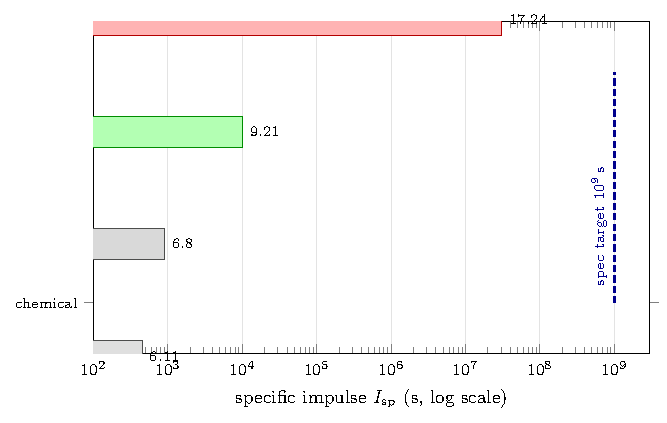
\includegraphics[width=0.82\linewidth]{figures/fig05_isp_ladder.pdf}
\caption{The specific-impulse ladder across propulsion classes, on a log
scale: chemical ($\sim\!450$\,s), nuclear fission/NTR
($\sim\!900$\,s), D--T fusion / MHD ($\sim\!10^4$\,s), and the antimatter
$\gamma$-rocket photon ceiling $I_{\text{sp,max}}=c/g\approx3.06\times10^7$\,s
(red, Eq.~\eqref{eq:s3-isp}). The spec target $10^9$\,s (grey dashed) sits
two decades \emph{above} the photon ceiling and is reachable only under the
fuel-mass effective-$I_{\text{sp}}$ definition (F-ANTI-3 closure). Stage-3
inherits the lowest-tier rung honestly: the $c/g$ ceiling is the
relativistic wall, not the spec number. Comparison values are
representative class anchors, not measured engine data (@D~g3).}
\label{fig:s3-isp-ladder}
\end{figure}

% -------------------------------------------------------------------------
\subsection{Honest scope}
\label{app:stage3-scope}

This appendix closes the relativistic energy bookkeeping of the
$\gamma$-rocket exhaust and the photon $I_{\text{sp}}$ ceiling, both as
exact recomputes ($|\Delta|=0$). It does not close the engine: the
directional $\gamma$-flux, the $5\pi$-sr shielding budget, antiproton
storage, and the wet-lab antihydrogen production rate are all downstream.
The $c/g$ ceiling is the load-bearing honest number; the F-ANTI-3 closure
reconciles a \emph{definition}, and is logged as such. Stage-3 remains a
\emph{feasibility witness} consistent with \texttt{absorbed=false}.
